\chapter{Modelling the economically viable wood in the crown of European beech trees}
\label{chap:beech_crowns}
{\large Kai Husmann$^1$ - Bernhard M�hring$^1$}\\

\vspace{3cm}
\noindent
$^1$University of G�ttingen, Department of Forest Economics and Forest Management\\
B�sgenweg 3, 37077 G�ttingen, Germany \\

\vspace{\fill}
\noindent
Published in:\\
\textit{Forest Policy and Economics} 78 (2017): 67-77 \\(DOI: 10.1016/j.forpol.2017.01.009)

\newpage
\begin{itemize}
	\item Bernhard M�hring supported analysis of the results, writing of the manuscript and the review process.
\end{itemize}

\clearpage
%%%%%%%%%%%%%%
%% Abstract %%
%%%%%%%%%%%%%%
\section*{Abstract}
\label{chap:beech_crowns:Abstract}
Long-term forest development programs in Germany aim on an increase of close-to-nature broadleaf forest stands. This means that the economic importance of European beech is expected to increase. The economic potential of a tree basically consists of the stem as well as the economically viable wood volume in the crown. Due to the high morphological variability of European beech crowns, taper models are often not satisfactory for predicting the economically viable wood volume arising from crowns. Prediction models with a higher precision are recently still lacking. Aim of this study is thus the development of prediction model for the economically viable crown wood volume of European beech trees.

We determined the distribution of the wood volume in the crown over the branch diameters using the multistage \textit{randomized branch sampling} method (RBS). The tree-specific wood volume distribution on the branch diameters were used to cluster all sampled trees into 3 groups. Additionally, we developed a method able to distinguish between economically viable and unviable crown branches. Basing on the RBS measurements as well as revenues and processing costs, we modeled the economically viable wood volume from the crown for each tree. To calculate the wood volume under bark, we parameterized a bark thickness function from disk samples of the trees.

We showed that the European beech crowns could be clustered into 3 groups differing in their wood volume distribution. The economically viable wood volume in the crown significantly depended on this grouping parameter as well as diameter at breast height (DBH). By contrast, the total amount of wood in the crown only depended on DBH. The differing viable wood volumes in the crowns were thus explained by different wood distributions and not by differing total crown wood volume. To make the results applicable in practice forestry, the modeling results were used to develop a regression formula able to predict the economically viable wood volume in the crown depending on the DBH and the crown type. As the crown type can also be predicted via measurable tree covariates, the regression model of the viable wood volume in the crown can be used as a support tool for the management of European beech stands. Sensitivity analysis quantifies how harvest revenues and costs translate into different viable tree volume.

\subsection*{Keywords}
Economically optimal wood cut, Crown morphology, European beech, viable crown wood, wood allocation, forest management

\subsection*{Highlights}
\begin{itemize}
\item Morphological measurements of 163 European beech tree crowns via \textit{RBS} method.
\item Distinguishing the economically viable from the whole crown wood.
\item Categorization of European beech crowns into morphological types.
\item Development of a viable crown timber prediction model for forest management.
\end{itemize}

%%%%%%%%%%%%%%%%%%
%% Introduction %%
%%%%%%%%%%%%%%%%%%
\section{Introduction}
\label{sec:beech_crowns:Introduction}
Although European beech (\textit{Fagus sylvatica} [L.]) forests have been identified as the dominant forest communities in the potential natural vegetation of Germany \citep{fanc_2010}, with 1,680,072 ha, they currently only account for 15 \% of Germany's forest stand cover \citep{ti_2014}. Long-term ecological forest development programs result in a general increase in deciduous tree species with a focus on European beech \citep{mfacp_2004}. The economic importance of European beech will thus further increase.

Traditionally the objective of European beech management is to maximize valuable stem wood \citep{nagel_2008}. Especially under the perspective of modern utilization methods like bio-economics \citep{hildebrandt_2014} and the increasing demand for fuel wood \citep{mantau_2012}, the economic importance of smaller branches of European beech is expected to increase. Thus a large proportion of the economic potential lies in smaller branches. Under certain conditions, further economic potential can be found in the tree stump and foliage \citep{miettinen_2014}. For a suitable management of European beech stands, it is necessary to assess the economically viable wood cut fully \citep{mohring_1997}. Therefore, as well as predicting the wood from the sympodial stem, it is also necessary to predict the economically viable wood cut in the sympodial crown. In the complex crowns of broadleaf trees, the economically viable wood can be substantially smaller than the whole wood volume. For this purpose, a model able to distinguish the economically viable wood volume from the whole wood volume in the crown is needed. For the stem volume prediction, there are many different and sophisticated tariff and other functions available. Cubic taper models exist, providing an adequate prediction of the economic potential of coniferous trees and the stems of deciduous trees \citep{kuzelka_2012}. However, those taper functions do not account for the complex sympodial form above the crown base of broadleaf tree species where the wood volume is not allocated around a throughout stem axis. They are therefore imprecise in predicting the wood volume arising above the crown base. They are usually calibrated for a minimum small-end diameter threshold of 7 cm. This small-end diameter can lack economic interpretation.

The aim of this study is to develop a parametric, practically usable prediction model of the economically viable wood volume in the crown of European beech trees. For this purpose, 163 beech trees were felled. Using the multistage \textit{Randomized Branch Sampling} (RBS) method \citep{gaffrey_1999}, a sound sample of branches was measured from each tree. The measurements were taken to examine the tree individual distribution of the wood volume in the crown on the crown branches. To develop tree individual morphological covariates, the sampled trees were clustered into groups with differing wood volume distribution. A multinomial regression model enables the prediction of this covariate via measurable tree attributes. We additionally developed a model, which predicts the viable wood volume from the measured wood volume distribution. This viable wood volume does not depend on freely selected but on economically justified small-end diameters. We developed a method to classify economically viable and unviable branches in European beech crowns via a break-even analysis. Then only the wood volumes of viable branches were estimated via RBS. The modeled economically viable wood volume thus depends on the size of the tree and the volume distribution in the crown. To calculate the wood volume under bark, we parameterized a new bark thickness function from disk samples of the trees.
To make the results applicable in forest practice, we performed a regression analysis with the modeled economically viable wood volume and further tree covariates. To ensure the applicability, we only used practically measurable tree attributes. The regression model represents a new approach for modeling the economic potential of European beech crowns and therefore a novel decision support tool for forest management operations.

%%%%%%%%%%%%%%%%%%%%%%%%%%%
%% Materials and Methods %%
%%%%%%%%%%%%%%%%%%%%%%%%%%%
\section{Materials and Methods}
\label{sec:beech_crowns:methods}
The dataset for this study comprised measurements from a destructive sample of 163 European beech trees sampled using the multistage RBS method \citep{gaffrey_1999, jessen_1955}. These data were compiled from 2 existing databases at the Northwest German Forest Research Station and the Baden-W�rttemberg Forest Research Centre.
%%-------------------------------------%%
%% Data sampling and sample processing %%
%%-------------------------------------%%
\subsection{Selection of trees}
\label{subsec:beech_crowns:methods:tree_selection}
The data were collected during 2009 and 2014. Altogether 163 trees were destructively sampled. In order to cover as many growth zones as possible, the sample plots were distributed throughout Germany (Figure \ref{fig:beech_crowns:fig1}). To ensure representation of the entire relevant diameter range, we chose up to 3 forest sites with different stand ages within these growth zones. All selected sites were high forests under standard management regimes. Depending on the area size of the plot, 2 - 4 sample trees were selected. In addition to the morphological measurements via RBS, DBH and tree height were measured (Table \ref{tab:beech_crowns:tab1}).

\begin{figure}
	\center
	\includegraphics[width=0.7\textwidth]{Grafiken/beech_crowns/Fig_1_plot_locations.eps}
	\caption{Sample site locations. Source of the background map: \citet{facg_2014}.}
	\label{fig:beech_crowns:fig1}
\end{figure}

\begin{table}[]
	\centering
	\caption{Summary statistics of the sampled trees. The sample size was 163.}
	\label{tab:beech_crowns:tab1}
	\begin{tabular}{cccc}
		\hline
		             &DBH             & height  & age \\ 
		             &[cm]            & [m]         &  [a] \\ \hline
		min          & 8.0            & 13.1        & 21      \\
		mean         & 35.4           & 25.3        & 85      \\
		median       & 34.8           & 26.0        & 80      \\
		max          & 78.3           & 38.5        & 180     \\ \hline
	\end{tabular}
\end{table}

%%--------------------%%
%% Selection of disks %%
%%--------------------%%
\subsection{Selection of disks}
\label{subsec:beech_crowns:methods:disk_selection}

To subtract bark from the wood volume, stem and branch disks for bark thickness measurement were taken from 37 trees of the NW-FVA study (Table \ref{tab:beech_crowns:tab2}). Up to 6 disks were randomly selected using the importance sampling method \citep{Gregoire_2008}. The proxy function, which is necessary for calculation of the sampling probability, was derived by the volume distribution of the branch diameters over the approximated tree height (which were both measured for volume estimation via RBS anyway). The selection probability of the disks was thus proportional to their disk diameter. Diameter and the bark thickness of the disks were measured at 4 directions of the selected disks directly after extraction.

\begin{table}[]
	\centering
	\caption{Summary statistics of disks for bark thickness measurements.}
	\label{tab:beech_crowns:tab2}
	\begin{tabular}{ccccccccccc}
		\cline{3-6} \cline{8-11}
		&  & \multicolumn{4}{c}{single bark thickness {[}mm{]}} &  & \multicolumn{4}{c}{disk diameter over bark {[}cm{]}} \\ \cline{1-1} \cline{3-6} \cline{8-11} 
		N   &  & min        & mean       & median       & max       &  & min        & mean        & median       & max        \\ \cline{1-1} \cline{3-6} \cline{8-11} 
		149 &  & 0.6        & 3.0        & 2.4          & 9.0       &  & 1.0        & 18.0        & 12.0         & 64.2       \\ \cline{1-1} \cline{3-6} \cline{8-11} 
	\end{tabular}
\end{table}

%%-----------------------%%
%% Selection of branches %%
%%-----------------------%%
\subsection{Selection of branches}
\label{subsec:beech_crowns:methods:branch_selection}
The estimation of the wood volume in the crown was based on the RBS method of multistage probability sampling. RBS is an unbiased method of probability sampling used for estimating specific tree parameters by measurable auxiliary variables \citep{jessen_1955,gaffrey_1999}. In our application, RBS enables estimation of the wood volume in the crown or in specific parts of the crown by measuring only a sample of branch segments instead of measuring all branch segments in the crown. Only relatively few measurements of branch diameters and branch segment lengths have to be taken for an accurate estimate of the whole wood volume in the crown or the wood volume of specific crown parts.

RBS is based on the knowledge of the conditional probability $q_{lj}$ of choosing the $j$-th out of n \textit{branches} at a \textit{node} $l$ in the crown instead of choosing another branch of this node. The probability $q_{lj}$ can be calculated by an auxiliary variable instead of the (complicated measurable) target variable itself \citep{gregoire_1995,Gregoire_2008,valentine_1984}. Instead of measuring the volume of all branches at a node, in our case, we only had to measure the base diameters $d_{lj}$ of the branches to calculate $q_{lj}$ and the volume of one branch. As \citet{west_1999} examined an allometric coefficient of 2.67 between branch volume and branch base diameter, the branch base diameter to the power of 2.67 is expected to provide efficient estimates. In our study, the conditional probability has been selected to be

\begin{equation}
	\label{eq:beech_crowns:eq1}
	q_{lj}(d)=d_{lj}^{2.67}/ \sum_{j=1}^{n_l} d_{lj}^{2.67}
\end{equation}

Thus once all branch base diameters $d_{li}$ at a node were recorded, one of the branches can be randomly chosen with probability $q_{lj}$. Only the \textit{segment} volume of this chosen branch has to be measured, where a \textit{segment} is defined as the part of the branch between 2 nodes \citep{Gregoire_2008}. We chose the formula for a conical frustum (Equation \ref{eq:beech_crowns:eq2}) to calculate the segment volume $v_{lj}$ via the branch base diameter $d_{lj}$, the base diameter at the following node $d_{lj+1}$ and the segment length $h_{lj}$. The volume of the following node $d_{lj+1}$ was also measured and added to the segment volume $v_{lj}$.

\begin{equation}
	\label{eq:beech_crowns:eq2}
	v_\mathit{lj}=\frac{h_{lj}\pi}{12}\left(d_{lj}^2+d_{lj}d_{{lj}+1}+d_{{lj}+1}^2\right)
\end{equation}

The crown base, which is the height where the throughout stem ends and the sympodial crown starts, represented the first node of the RBS procedure. To have a measurable criterion, we defined the crown base to be the tree height where a branch base diameter was > 1/5 of the stem diameter at that height. A whole RBS path thus consisted of a succession of randomly selected branch segments from the crown base up to one shoot bud. Along the path all branch base diameters and all segment volumes were measured. In order to get an idea of the variation, 3 random and distinct RBS paths were obtained for each of the 163 sampled trees.

%%--------------------------------------------------------%%
%% Estimation of wood volume in the stem and in the crown %%
%%--------------------------------------------------------%%
\subsection{Estimation of wood volume in the stem and in the crown}
\label{subsec:beech_crowns:methods:crown_vol_est}
The calculation method for the point estimates of the volumes as well as for the estimated variance is described in the literature \citep[e. g.][]{Gregoire_2008}. The stem form was assessed by section-wise diameter measurements at certain tree heights up to the crown base. The sum of these section volumes, also calculated by the conical frustum formula (Equation 2), gave the whole stem volume from the ground up to the crown base.

%%----------------------------------------------%%
%% Economically viable wood volume in the crown %%
%%----------------------------------------------%%
\subsection{Economically viable wood volume in the crown}
\label{subsec:beech_crowns:methods:viable}

%%++++++++++++++++++++++++++++%%
%% Crown type differentiation %%
%%++++++++++++++++++++++++++++%%
\subsubsection{Crown type differentiation}
\label{subsubsec:beech_crowns:methods:viable:crown_types}
To calculate the volume distribution according to the branch diameters in individual tree crowns, the cumulative wood volume amount $\hat{V}_i(d)$ in the crown was calculated from the crown base up to each recorded branch base diameter $(d)$ along each RBS path. This distribution was normalized by dividing the predicted cumulative crown volume below $\hat{V}_i(d)$ [m3] by the whole wood volume from the crown $\hat{V}_i(0)$ [m3] (Equation \ref{eq:beech_crowns:eq3}) and by dividing the base diameter of every branch $d_{ij}$ by the maximum diameter found $d_{max}$. $F(d)$ thus denotes the wood volume amount over branch diameter in the crown.

\begin{equation}
\label{eq:beech_crowns:eq3}
F\left(d\right)=\frac{{\widehat V}_i\left(d\right)}{\widehat V}
\end{equation}

The diameter where half of the wood volume amount was located above (below respectively) was interpreted as the median branch diameter of a tree crown. This median volume branch diameter $F(d_{0.5})$ was easily interpolated from the generated diameter distribution for every RBS path, where $d_{0.5}$ denotes the branch diameter for which $F(d_{0.5})=0.5*F(d_{max})$. The same appears for the lower $F(d_{0.25})$ and upper quantile $F(d_{0.75})$. The curve trend of $F(d)$ over branch diameter thus indicates whether most of the wood volume is located in relatively small or in larger branches. Generally, there were 3 types of volume distribution in the data (Figure \ref{fig:beech_crowns:fig2}). The first type showed a high share of volume in relatively small branch dimensions (left). The median branch diameter of these trees was close to the lower quantile. In the balanced type (center), half of the wood volume was found above a branch diameter that was approximately half the size of the largest diameter of the respective tree. In the third type (right), major part of wood volume was allocated in the larger branch diameter range. The median diameter was close to the upper quantile.

\begin{figure}
	\center
	\includegraphics[width=1\textwidth]{Grafiken/beech_crowns/Fig_2_relative_volume_amount.eps}
	\caption{Cumulative crown wood volume over relative branch diameter for 3 exemplary trees. For each tree all 3 RBS paths are displayed. The diameters where half of the timber volume is located above, respective below (the median relative branch diameter) are marked by vertical lines.}
	\label{fig:beech_crowns:fig2}
\end{figure}

As there were 3 paths per tree, the tree individual median diameter was calculated by the median of the 3 median branch diameters. The lower and upper quartiles were created in the same way. We thus generated 3 tree individual continuous variables. These enabled a clustering of the trees into 3 crown types which differ in their wood volume amount. As the crown types based on the volume distribution in the crowns, they should represent groups with different economically viable wood volumes. We chose the \textit{k-means} cluster algorithm \citep{r_core_team_2016}, which minimizes the within-cluster Euclidean distance among observations and group means by the sum-of-squares method \citep{wagstaff_2001}, to cluster the data into 3 morphological crown types.

The median tree diameter as well as the quantile tree diameters are not measurable in practice. To differentiate a beach crown into 1 of the 3 mentioned groups in forest management, it is thus necessary to predict the crown type by other tree attributes. A multinomial logistic regression method \citep{hutcheson_2008} was parameterized to predict the crown type clusters from practically measurable morphological tree variables $x_i$ (equation 4). In this case, the $x_i$ are the DBH, the tree height, the tree height at crown base and the ratio of the base diameters at crown base. The ratios of the branch diameters at crown base were calculated by dividing the 2nd largest base diameter at the crown base by the respective largest branch diameter.

We fitted a log odd model with $J=3$ categories to a probability function which predicts the probability that an individual tree is belonging to a crown type category $j$ rather than to the reference category $j^{'}= 1$ by $i=4$ variables.

\begin{equation}
\label{eq:beech_crowns:eq4}
\operatorname{log}\left(\frac{P\left(Y=j\right)}{P\left(Y=j^{'}\right)}\right)=\beta_{j0}+\beta_{j1}x_{1}+\beta_{j2}x_{2}+\dots+\beta_{ji}x_{i}
\end{equation}

The probability of an individual to belong to group j in relation to the reference is therefore calculated as

\begin{equation*}
P\left(Y=j\right)=\frac{\operatorname{exp}\left(\beta_{0}+\beta_{j1}x_{1}+\beta_{j2}x_{2}+\dots+\beta_{jk}x_{k}\right)}{1+\operatorname{exp}\left(\beta_{0}+\beta_{j1}x_1+\beta_{j2}x_{2}+\dots+\beta_{jk}x_{k}\right)}=\frac{exp(\boldsymbol{x}_i^{'}\boldsymbol{\beta}_j)}{1+exp(\boldsymbol{x}_i^{'}\boldsymbol{\beta}_j)}
\end{equation*}

and the probability of an individual to belong to group j considering all groups calculates as

\begin{equation*}
P\left(Y=j\right)=\frac{exp(\boldsymbol{x}_i^{'}\boldsymbol{\beta}_j)}{1+\sum_{s=1,s\neq j'}^{J} exp(\boldsymbol{x}_i^{'}\boldsymbol{\beta}_s)}
\end{equation*}

where crown type 1 represented the reference category $j^{'}$. The model was fitted with the R package \textit{NNET} \citep{venables_2002}. The significance of a variable was examined by linear discriminant analysis. For model quality testing we predicted the crown type with our model and compared the result with the actual crown classification by the k-means analysis. This classification was performed by a leave-one-out cross-validation \citep[R package \textit{MASS};][]{venables_2002} and an in-sample reclassification.
%%++++++++++++++++++++++++++++++++++++++++++++++++++++++++++++%%
%% Modelling the economically viable wood volume in the crown %%
%%++++++++++++++++++++++++++++++++++++++++++++++++++++++++++++%%
\subsubsection{Modelling the economically viable wood volume in the crown}
\label{subsubsec:beech_crowns:methods:viable:econ_viable}
As biasedness of the point and the variance estimate do not depend on the number of stages, RBS also allows the volume estimation of specific parts in the crown \citep{cancino_2005}. We used this property to estimate the tree individual viable wood volume in the crown only. For this, we programmed a model that distinguished the economically viable from economically unviable branches in the RBS sample (Algorithm \ref{alg:beech_crowns:alg1}). After running the algorithm, only the economically viable branches were then used to estimate the wood volume via the RBS method. The predicted wood volume after application of the separation algorithm thus reflected the economically viable wood volume in the crown.

To distinguish viable from unviable branches, each RBS node and subsequent selected branch segment were aggregated into one \textit{branch structure}. In the event that many nodes occurred in close succession (no branch segments in between), they were regarded as one large node and aggregated with the following node and branch segment to form a large branch structure.

Each of the branch structures were then, starting at the crown base, successively rated in terms of revenue and cost. The revenue was calculated by multiplying wood volume [$\text{m}^3$] (under bark) by timber price [$\text{\euro} \text{m}^{-3}$]. The cost associated with any one branch structure was assumed to be constant per processing step and was interpreted as marginal cost \citep{mohring_1997} of processing this branch structure. Whenever a branch structure had a positive marginal return, it was additionally proofed if the former branch structure was viable. If this was the case, the branch structure was labeled to be economically viable. A branch segment is thus only considered as economically viable if its piece-volume is large enough to have a positive marginal return. If a former branch structure was unviable, the processing costs doubled, because the continuation of processing thereafter would require an additional cut. Each RBS path of every crown thus had a specific break-even point \citep{starr_1975} after which further processing would result in lower marginal returns. The small-end diameter of this last viable branch structure was recorded. The model was programmed in the statistical programming language R \citep{r_core_team_2016}.

After neglecting the unviable branch structures, the tree individual viable wood volume from the crown as well as the variance were estimated by means of RBS. The final small-end diameter of an individual tree was defined as the mean of the end diameter of all 3 paths.

\begin{algorithm}[H]
	initialization of processing $costs$ and $revenue$ by the user\\
	aggregation of the RBS $knots$ and $branch$ $segments$ into $structures$ \\
	\hfill \\
	\For{i in (1 : $N_{paths}$)}{
		\For{j in (1 : $N_{structures}$)}{
			\eIf{volume of $structure_{ij}*revenue > processing$ costs}
			{\eIf{$economical$ $viability$ $of$ $structure_{ij-1}$==TRUE}
				{$economical$ $viability$ $of$ $structure_{ij} \leftarrow TRUE$ \\
					$small-end$ $diameter_j$ $\leftarrow$ $end$ $diameter$ $of$ $structure_{ij}$}{
					\eIf{volume of $structure_{ij}*revenue > processing$ $costs*2$}
					{$economical$ $viability$ $of$ $structure_{ij} \leftarrow TRUE$ \\
						$small-end$ $diameter_j$ $\leftarrow$ $end$ $diameter$ $of$ $structure_{ij}$}
					{$economical$ $viability$ $of$ $structure_{ij} \leftarrow FALSE$}}
			}
			{$economical$ $viability$ $of$ $structure_{ij} \leftarrow FALSE$}
		}
	}
	\hfill \\
	$crown$ $timber$ $volume$ $\leftarrow$ RBS estimation of the viable structures \\
	$variance$ $\leftarrow$ RBS estimation of the viable structures\\
	$small$-$end$ $diameter$ $\leftarrow$ mean($small$-$end$ $diameter_1$, $...$, $small$-$end$ $diameter_{N_{paths}}$)
	\\
	\hfill \\
	
	\textbf{return} ($crown$ $timber$ $volume$, $variance$, $small$-$end$ $diameter$) \\
	\caption{Pseudocode of the of the economically viable wood volume distinguishing model where $N_{paths}$ is the number of paths per tree (in this study always 3) and $N_{structures}$ is the number of branch structures per path.}
	\label{alg:beech_crowns:alg1}
\end{algorithm}

The model (Algorithm \ref{alg:beech_crowns:alg1}) thus needed timber price [$\text{\euro} \; \text{m}^{-3}$] (under bark) and marginal costs [$\text{\euro} \; \text{processing step}^{-1}$] as input parameters. It was parameterized with commonly used values to ensure realistic results. The revenue was set to 50 $\text{\euro} \; \text{m}^{-3}$ (under bark) to reflect the common price for industrial wood in Germany in 2016 \citep{degenhard_2016}. The fixed cost parameter was based on the European beech wages table from the forest entrepreneurs association \citep{haarhaus_2012}, which assumes an 125 \% entrepreneur fee and 19 \% value added tax. Based on the assumptions that each node occurring represented one processing step and that the costs of each were constant, the costs amounted to 0.35 $\text{\euro} \; \text{processing step}^{-1}$. The model outputs were the economically viable wood from the crown (under bark) [$\text{m}^3$] and small-end diameter [mm].

\begin{equation}
\label{eq:beech_crowns:eq5}
\begin{aligned}y&=\beta\prod_{i=1}^kx_i^{\alpha_i}\\\leftrightarrow\operatorname{log}\left(y\right)&=\operatorname{log}\left(\beta\right)+\sum_{i=1}^k\alpha_i\operatorname{log}\left(x_i\right)\end{aligned}
\end{equation}

The modeled viable wood volumes were used to parameterize an allometric growth model (Equation \ref{eq:beech_crowns:eq5}) with $k$ covariates. This parametric regression model allows forecasting of the economically viable crown wood volume by measurable covariates and is therefore easily applicable in forest management. For this purpose, sets of results, differing in their parameterization of input variables, were generated with the viable wood volume prediction model (Algorithm \ref{alg:beech_crowns:alg1}). The revenue as well as the cost input parameters were firstly set to the common parameter combination (50 $\text{\euro} \; \text{m}^{-3}$, 0.35 \euro \; $\text{step}^{-1}$) and then separately changed by 20 \%. Altogether, there were 9 result sets generated where each set of results involved 163 datasets. Because there were void datasets, whenever the algorithm assigned no viable wood volume in the crown, the data reduced to 1347 datasets. The regression analysis was composed of the covariates DBH, tree height, tree height at crown base, crown width, diameter ration at crown base and tree age as well as crown type, revenue scenario and cost scenario, which both functioned as dummy variable. The dependent variable was the modeled economically viable wood volume in the crown. The significance analysis and the model parameterization were performed by a \textit{generalized linear model} \citep[R Package \textit{stats};][]{r_core_team_2016}. Proof of the significant impact of the covariates on $\alpha$ was not possible due to insufficient crown type 3 observations in larger DBH dimensions. The significance analysis was thus performed on $\beta$. Linearity and homoscedasticity were achieved by a Gamma distributed log-link function \citep{wood_2006}.
%%--------------------------%%
%% Allometric relationships %%
%%--------------------------%%
\subsection{Allometric relationships}
\label{subsec:beech_crowns:methods:allo}
In the metabolic scaling theory, the relationship between two plant organs ($y$ and $x$, see also Equation \ref{eq:beech_crowns:eq5}) can be described by a power law \citep{huxley_1932,niklas_1994}. This power law interprets the intraspecific relationship between plant organs for a given species. The variability of the relationship describes the strength of the allometry \citep{pretzsch_2010,west_1997}. Allometric model are thus useful to investigate the relationship between variables of economic interest and further tree attributes.

To consider the assumption of allometric regressions \citep{stumpf_2012}, we transformed the data by taking the natural logarithm. The relationships were regressed with the \textit{standardized major axis} method \citep[R package \textit{SMATR};][]{warton_2012}. The retransformation bias was estimated and corrected from the residual standard error of the log linear model \citep{sprugel_1983}.
%%%%%%%%%%%%%
%% Results %%
%%%%%%%%%%%%%
\section{Results}
\label{sec:beech_crowns:results}

%%------------------------------%%
%% Estimation of bark thickness %%
%%------------------------------%%
\subsection{Prediction of bark thickness}
\label{subsec:beech_crowns:results:bark}
To subtract the bark from the wood volume, models for the double bark thickness over branch diameter are necessary. The predicted double bark thickness enabled the bark subtraction from both sides of the RBS diameter measurements. The commonly used double bark thickness model of \citet{altherr_1978} was parameterized with stem and branch disks of diameters above 7 cm. As the wood volume model in this study should be able to predict smaller branches as well, parameterization of an own bark thickness model became necessary. In addition, comparison of the observed bark thickness to the predicted bark thickness with the equation by \citet{altherr_1978} revealed that application of the Altherr model would have led to an overestimation of the bark thickness. The estimated double bark thickness with the function by \citet{altherr_1978} was 1.4 mm higher than with the new parameterized function for branches with a diameter of 10 cm. For branches with diameter of 30 cm, the difference amounted to 3.1 mm.

The double bark thickness regression equation was calculated via a \textit{Generalized Additive Mixed Model} \citep{wood_2006} using the untransformed normally distributed identity link function. A linear curve trend was found in the bark thickness model (Fig \ref{fig:beech_crowns:fig3}). There were multiple measurements in one tree (see section \ref{subsec:beech_crowns:methods:disk_selection}). To exclude regional as well as tree specific influences, the tree id was considered a random effect. As we found heteroscedasticity, we weighted our data by a power function, which was parameterized by the model residuals over the fitted values.

\begin{figure}
	\center
	\includegraphics[width=0.5\textwidth]{Grafiken/beech_crowns/Fig_3_bark_thickness.eps}
	\caption{Double bark thickness over disk diameter (over bark) and the fitted linear bark thickness model.}
	\label{fig:beech_crowns:fig3}
\end{figure}

The model (Table \ref{tab:beech_crowns:tab3}) represented a valid method for subtracting bark from both sides of every morphological RBS diameter measurement. The volume calculation after bark subtraction via RBS thus predicts the volume under bark. This was also done for the section-wise stem diameter measurements to predict the stem wood volume under bark.

\begin{table}[]
	\centering
	\caption{Summary statistics of the linear double bark thickness [mm] regression model. Independent variable is the diameter over bark [cm] (fresh).}
	\label{tab:beech_crowns:tab3}
	\begin{tabular}{ccccc}
		\hline
		variable             & coefficient & standard error & t-value & p-value          \\ \hline
		intercept            & 1.87804     & 0.25           & 7.42    & \textless2*10-16 \\
		diameter             & 0.23253     & 0.01           & 16.06   & \textless2*10-16 \\ \hline
		observations         & 149         &                &         &                  \\
		AIC                  & 565.0       &                &         &                  \\
		model range {[}cm{]} & 0 - 65      &                &         &                  \\ \hline
	\end{tabular}
\end{table}

%%----------------------------------------------%%
%% Economically viable wood volume in the crown %%
%%----------------------------------------------%%
\subsection{Economically viable wood volume in the crown}
\label{subsec:beech_crowns:results:viable}

%%++++++++++++++++++++++++++++%%
%% Crown type differentiation %%
%%++++++++++++++++++++++++++++%%
\subsubsection{Crown type differentiation}
\label{subsubsec:beech_crowns:results:viable:crown_types}
All calculated and measured crown morphology variables and tree metadata, including mean coefficient of variation for the data estimated by the RBS method, are summarized in Table \ref{tab:beech_crowns:tab4}. The crown type classification analyses were based on the median branch diameter and the branch diameter quartiles. The other tree variables were then used to parameterize a prediction model for the crown type classes.

\begin{table}[]
	\centering
	\caption{Summary statistics of all used variables, c. v. = coefficient of variation.}
	\label{tab:beech_crowns:tab4}
	\begin{tabular}{cccccccc}
		\hline
		variable                       &                            & unit     & min   & median & mean  & max    & c. v. \\ \hline
		diameter at breast height      & $DBH$                        & {[}cm{]} & 8.0   & 34.8   & 35.4  & 78.3   & -     \\
		tree height                    & $H$                          & {[}m{]}  & 13.1  & 26.0   & 25.3  & 38.5   & -     \\
		whole tree wood volume         & $V_t$                       & [$\text{m}^3$] & 0.05 & 1.46  & 2.25 & 11.70 & 0.07 \\
		crown wood volume              & $\hat{V}_i(0)$ & [$\text{m}^3$] & 0.01 & 0.64  & 1.21 & 9.20  & 0.22 \\
		tree wood volume (u. b.) & $V_{tub}$                     & [$\text{m}^3$] & 0.04 & 1.36  & 2.11 & 10.98 & 0.07 \\
		crown wood volume (u. b.)      & $V_{cub}$                    & [$\text{m}^3$] & 0.01 & 0.59  & 1.12 & 8.62  & 0.22 \\
		median branch diameter         & $F(d_{0.5})$                 & [$\text{m}^3$] & 23  & 138  & 152 & 406  & -     \\
		height at crown base           & $CB$                         & {[}m{]}  & 1.6   & 10.9   & 10.8  & 21.1   & -     \\
		diameter ratio at crown base   & $DR$                         & -        & 0.2   & 0.4    & 0.4   & 0.9    & -     \\ \hline
	\end{tabular}
\end{table}

The trees were clustered into 3 groups, where 50 trees were assigned to the first (bulk of volume in smaller branches), 69 to the second (balanced volume allocation) and 44 to the third (bulk of volume in larger branches) crown type. As median and quantile tree diameters cannot be measured practically but the model shall be applicable in forest management, the influence of measurable variables on the crown types was assessed. The influence of tree attributes on the crown type was tested by linear discriminant analysis \citep{venables_2002}, analysis of variance and deviance \citep{chambers_1992} as well as analysis of Akaike Information Criterion \citep{akaike_1981}. Only significant variables and interactions were chosen as regression parameters (Table 5). The analysis of variance revealed the significance of the diameter ratio at crown base $DR$. Deviance of the residuals (310.3 without $DR$) as well as AIC (330.0 without $DR$) were also substantially improved by this variable. Due to their high linear correlation with the significant variables, tree age and crown width were insignificant. The model is applied by plugging the coefficients of Table \ref{tab:beech_crowns:tab5} into Equation \ref{eq:beech_crowns:eq4}.

\begin{table}[]
	\centering
	\caption{Summary statistics of the multi-nominal logistic crown type prediction model with independent variables DBH [cm], tree height (H) [m], height at crown base (CB) [m] and branch diameter ratio at crown base (DR) including the results of the leave-one-out cross-validation (c.-v.) and the within-model reclassification (w.-m.).}
	\label{tab:beech_crowns:tab5}
	\begin{tabular}{ccccccc}
		\cline{3-4} \cline{6-7}
		&   & \multicolumn{2}{c}{crown type 2}   &   & \multicolumn{2}{c}{crown type 3}  \\ \cline{1-1} \cline{3-4} \cline{6-7} 
		variable   &   & coefficient    & standard error    &   & coefficient    & standard error   \\ \cline{1-1} \cline{3-4} \cline{6-7} 
		intercept  &   & 10.3679421     & 0.005             &   & 20.39087       & 0.011            \\
		DBH        &   & -0.4522104     & 0.105             &   & -0.8534910     & 0.164            \\
		H          &   & -0.2423880     & 0.096             &   & -0.3248841     & 0.130            \\
		CB         &   & -0.1208192     & 0.083             &   & -0.2971321     & 0.108            \\
		DR         &   & -20.1534122    & 0.006             &   & -31.3965027    & 0.005            \\
		DBH*H      &   & 0.0156519      & 0.003             &   & 0.0244615      & 0.004            \\
		DBH*DR     &   & 0.7159227      & 0.179             &   & 0.5762532      & 0.368            \\
		H*DR       &   & 0.6833604      & 0.143             &   & 1.0091659      & 0.242            \\
		DBH*H*DR   &   & -0.0266986     & 0.005             &   & -0.0218313     & 0.007            \\ \hline
		\multicolumn{6}{c}{number of observations}                               & 163              \\
		\multicolumn{6}{c}{AIC}                                                  & 312.0            \\
		\multicolumn{6}{c}{residual deviance}                                    & 276.9            \\
		\multicolumn{6}{c}{proportion of correct classified crown types (c.-v.)} & 0.50             \\
		\multicolumn{6}{c}{proportion of correct classified crown types (w.-m.)} & 0.56             \\ \hline
	\end{tabular}
\end{table}

%%++++++++++++++++++++++++++++++++++++++++++++++++++++++++++++%%
%% Modelling the economically viable wood volume in the crown %%
%%++++++++++++++++++++++++++++++++++++++++++++++++++++++++++++%%
\subsubsection{Modelling the economically viable wood volume in the crown}
\label{subsubsec:beech_crowns:results:viable:econ_viable}
Table \ref{tab:beech_crowns:tab6} shows that crown type 3 crowns yielded more economically viable wood volume than the other two types for trees with similar DBH. The percentage volume of economically viable wood modeled in relation to the whole wood volume from the crown was considerably different among the crown types. Especially crowns of type 3 differed from the other 2 types. The small-end diameter of the trees did not differ between the diameter-crown type-groups from Table 6. In all DBH-crown type-groups, except for the groups below 20 cm, the group mean of the small-end diameter was randomly scattering around 10 cm. Trees in the groups below 20 cm DBH usually don't show crown branches with a base diameter of 10 cm. Their group mean small-end diameter was not calculated.

\begin{table}[]
	\centering
	\caption{Proportion of economically viable crown wood in beech crowns according to the whole crown wood (each under bark). n. d. = no data.}
	\label{tab:beech_crowns:tab6}
	\begin{tabular}{ccccccccc}
		\cline{2-9}
		\multicolumn{1}{l}{} & \multicolumn{8}{c}{DBH-interval {[}cm{]}}                                                    \\ \cline{2-9} 
		crown type           & {[}0-10) & {[}10-20) & {[}20-30) & {[}30-40) & {[}40-50) & {[}50-60) & {[}60-70) & {[}70-80) \\ \hline
		1                    & n .d.    & 0.19      & 0.35      & 0.57      & 0.71      & 0.74      & 0.84      & 0.80      \\
		2                    & 0.00     & 0.25      & 0.42      & 0.65      & 0.72      & 0.71      & 0.84      & 0.80      \\
		3                    & 0.08     & 0.27      & 0.57      & 0.77      & 0.88      & 0.86      & 0.89      & n. d.     \\ \hline
	\end{tabular}
\end{table}

The model output data revealed that the return per $\text{m}^3$ substantially differs between the crown types (Figure \ref{fig:beech_crowns:fig4}). Trees with crowns of the type 3 showed in mean highest returns per $\text{m}^3$ while crowns of the type 1 were by trend lowest marginal returns over the entire observed diameter range.

\begin{figure}
	\center
	\includegraphics[width=0.5\textwidth]{Grafiken/beech_crowns/Fig_4_marginal_return.eps}
	\caption{Marginal return divided by volume (under bark) versus DBH differentiated by crown types.}
	\label{fig:beech_crowns:fig4}
\end{figure}

For sensitivity analysis of the model, the arithmetic mean of the economically viable wood volume from the crown (under bark) was calculated with all 163 trees (Figure \ref{fig:beech_crowns:fig5}, left). The reference was the common scenario (revenue: 50 $\text{\euro} \; \text{m}^{-3}$, costs: 0.35 $\text{\euro} \; \text{processing step}^{-1}$). Changes in costs as well as changes in revenues of 20 \% led to a change of the mean predicted crown wood volume up to 5 \%. Decreasing of revenues and costs affected the economically viable crown wood volume slightly more than respective increasing. The small-end diameter (at which cutting was stopped) was influenced by changing costs and revenues as well (Figure \ref{fig:beech_crowns:fig5}, right). With values ranging from 5 to 16 cm, the median small-end diameter of the common scenario was ca. 10 cm. 20 \% increasing costs increased the small-end diameter to a median of 11 cm with values ranging from 6 to 16 cm. 20 \% decreasing costs led to small-end diameters ranging from 5 to 15 cm with median 9 cm. By 20 \% increasing revenues decreased the median of the small-end diameters to 9 cm. Respective increasing of the costs led to a median small-end diameter of 11 cm. While differing costs as well as differing revenues led to a substantial change of the median small-end diameters, the distributions of the small-end diameters around the median were always approximately unchanged. The distribution of each scenario was symmetric with 1.5 quantiles ranging ca. 6 cm around the median. It additionally became obvious that simultaneous changing of costs and revenues did not change the median small-end diameter as well as the distribution around the median (Figure \ref{fig:beech_crowns:fig5}, right). The economically viable wood volume as well as the median small-end diameter thus only changed when one of the input variable changes while the respective other stays constant or changes in the opposite direction.

\begin{figure}
	\center
	\includegraphics[width=0.49\textwidth]{Grafiken/beech_crowns/Fig_5_left_elasticity_cost_revenue.eps}
	\includegraphics[width=0.49\textwidth]{Grafiken/beech_crowns/Fig_5_right_small-end_diameter_boxplot.eps}
	\caption{Relative change in the predicted economically viable crown timber volume over relative changes in costs and revenues (left) and the distribution of the small-end diameters at cost and revenue changes of 20 \% (right).}
	\label{fig:beech_crowns:fig5}
\end{figure}

The economically viable crown wood volume of European beech [m$^3$] (under bark) $V_v$, modeled with the introduced algorithm, was fitted to the exponential growth function (see Equation \ref{eq:beech_crowns:eq5}). The regression depended only on the covariate DBH $d$ [cm] and the crown type, which functions as dummy variable $ct_i$. Following Equation \ref{eq:beech_crowns:eq5}, the growth function can be written as

\begin{equation}
\label{eq:beech_crowns:eq6}
V_v = exp \left( log \left( \beta \right) + d_{\mathit{ct}1} \gamma_{\mathit{ct}1}+d_{\mathit{ct}3}\gamma_{\mathit{ct}3}\right)\mathrm{DBH}^\alpha
\end{equation}

The parameters values are shown in Table \ref{tab:beech_crowns:tab7}. $d_{ct1}$ and $d_{ct2}$ are dummy-variables. They are 1, if the volume of the respective crown type is to be predicted. If the volume of crown type 2 is to be predicted, both dummy variables must be set to 0. All further continuous covariates did not lead to a significant model improvement. Cost as well as revenue changes of 20 \% were partially significant. However, the dimension of these variables in comparison to the crown type dummy variables were low and the improvement of the AIC (-1027.3) was thus only very slight. Altogether, the slight model improvement does not justify consideration of the abstract and non-measurable cost and revenue change dummy variables. They were not chosen as model parameters. The same was found for cost and revenue changes up to 30 \%.

The difference between economically viable wood volume of crown type 1 and 2 was comparatively low (Table \ref{tab:beech_crowns:tab7}), whereas the difference between crown type 2 and 3 was approximately 20 \%.

\begin{table}[]
	\centering
	\caption{Summary of the economically viable crown wood volume regression model. The data was fitted to a natural exponential function by the generalized nonlinear regression method with the independent variables DBH and the crown type.}
	\label{tab:beech_crowns:tab7}
	\begin{tabular}{cccc}
		\hline
		variable               & coefficient & standard error & t-value \\ \hline
		log($\beta$)           & -13.30117   & 0.114          & -116.57 \\
		$\gamma_1$             & -0.06699    & 0.031          & -2.19   \\
		$\gamma_3$             & 0.19360     & 0.034          & 5.73    \\
		$\alpha$               & 3.48463     & 0.031          & 112.7   \\ \hline
		number of observations & \multicolumn{3}{c}{1347}               \\
		deviance explained     & \multicolumn{3}{c}{0.89}               \\
		model range {[}cm{]}   & \multicolumn{3}{c}{0-78 }              \\
		AIC                    & \multicolumn{3}{c}{-1022.9}            \\ \hline
	\end{tabular}
\end{table}

%%--------------------------%%
%% Allometric relationships %%
%%--------------------------%%
\subsection{Allometric relationships}
\label{subsec:beech_crowns:results:allo}
The whole tree and crown wood volume both revealed an allometric relationship to DBH (Figure \ref{fig:beech_crowns:fig6}a and b). Both relationships showed heteroscedasticity in the untransformed, and homoscedasticity on the double log transformed scale. The coefficients of determination of the relationships were very high, whereby the coefficient of determination of the crown wood volume-DBH relationship was slightly lower. There were no differences between the clustered crown types. The whole crown volume did not depend on the crown type (Table \ref{tab:beech_crowns:tab7}).

\begin{figure}
	\center
	\includegraphics[width=1\textwidth]{Grafiken/beech_crowns/Fig_6_allometric_relationships.eps}
	\caption{Allometric relationships of the whole aboveground wood volume (a), the crown wood volume (b) and the median branch diameter (d) over DBH as well as crown wood volume over total aboveground timber volume (c) incl. the back transformed regression function. The small windows show the logarithmic transformed data and the log linear regression function.}
	\label{fig:beech_crowns:fig6}
\end{figure}

Crown wood volume was found to increase disproportionally high with whole aboveground wood volume (c). Further, relationships like tree height-DBH and median branch diameter-DBH (d) showed a lower coefficient of determination and thus a higher variance than the former relationships (Figure \ref{fig:beech_crowns:fig6}a, b and c).

\begin{table}[]
	\centering
	\caption{Summary of the log linear regression models, fitted by the SMA method. $\alpha$ and log($\beta$) are the model coefficients; l.ci.lim is the lower, u.ci.lim the upper limit of the 95 \% confidence interval; r$^2$ is the linear coefficient of determination.}
	\label{tab:beech_crowns:tab8}
	\begin{tabular}{cccccc}
		\hline
		allometry                  & $\alpha$ & l.ci.lim & u.ci.lim & log($\beta$) & r$^2$ \\ \hline
		$V_f \propto DBH^{\alpha}$ & 2.492    & 2.444    & 2.541    & -8.408       & 0.98  \\
		$V_c \propto DBH^{\alpha}$ & 2.915    & 2.812    & 3.022    & -10.661      & 0.95  \\
		$V_c \propto V_f^{\alpha}$ & 1.170    & 1.131    & 1.209    & -0.821       & 0.95  \\
		$H \propto DBH^{\alpha}$   & 0.490    & 0.448    & 0.536    & 1.519        & 0.67  \\
		$MB \propto DBH^{\alpha}$  & 1.179    & 1.091    & 1.275    & 0.842        & 0.74  \\ \hline
	\end{tabular}
\end{table}


%%%%%%%%%%%%%%%%
%% Discussion %%
%%%%%%%%%%%%%%%%
\section{Discussion}
\label{sec:beech_crowns:discussion}

%%------------------------------%%
%% Estimation of bark thickness %%
%%------------------------------%%
\subsection{Estimation of bark thickness}
\label{subsec:beech_crowns:discussion:bark}
The most commonly used linear bark thickness function by \citet{altherr_1978} is only valid for branches with diameter > 7 cm. Since our viable wood volume should be able to predict smaller branches as well, the function by Altherr et al. was not applicable for our purposes. Furthermore, biomass thickness is known to have regional differences \citep{bonyad_2012}. As Alterr et al. collected their data in the southwest of Germany only, application of their model could lead to wrong predictions. Actually the function by Altherr et al. would have let to an overestimation of our measured bark thicknesses. 
Application of our new parametrized bark thickness model in further studies appears to be useful whenever regionalized functions are not available or when bark thicknesses of smaller branches (diameter < 7 cm) have to be predicted.

%%----------------------------------------------%%
%% Economically viable wood volume in the crown %%
%%----------------------------------------------%%
\subsection{Economically viable wood volume in the crown}
\label{subsec:beech_crowns:discussion:viable}
The mains advantage of the RBS method are its unbiasedness, its efficiency and its flexibility. Based on the morphologic measurements, it is possible to estimate the volume of various parts of the crown. In our approach, we focused on the economically viable branch structures. Although the measurements for this study were relatively time and cost expensive they represent an efficient trade-off between accuracy and measuring costs.

%%++++++++++++++++++++++++++++%%
%% Crown type differentiation %%
%%++++++++++++++++++++++++++++%%
\subsubsection{Crown type differentiation}
\label{subsubsec:beech_crowns:discussion:viable:crown_types}
The different types of volume distributions according to the branch diameters in the crowns $F(d)$ (Figure \ref{fig:beech_crowns:fig2}) indicate that different harvesting volumes in the tree crowns can be caused by the wood allocation. It is, from a practical perspective, immediately apparent that crowns with more wood volume in relatively large branch dimensions lead to higher yields than crowns with a lot of wood volume in relatively small branch dimensions. Branches with larger dimensions lead to lower procession costs per cubic meter \citep{neumann-spallart_1952}. While the variability in the cumulative volume is high, the general curve tends to be uniform over all trees (Figure \ref{fig:beech_crowns:fig2}).

To create a variable which is able to describe this economically relevant branch dimension numerically, the median and quantile diameter were calculated from the volume distribution of the branch diameter $F(d)$. Since a major part of the wood volume in type 1 crowns is allocated to relatively small branches and twigs, this crown type is the economically unfavorable in comparison to the other types. Classification of crown type appears to be a great advantage in forest planning as it enables a more accurate evaluation of the expectable wood amount from the crown of a tree.

The median and the quartiles of branch diameters are suitable for crown type classification but, unfortunately, they are not practically measurable. For this purpose, after the classification via median and quantile branch diameters, further relationships between tree parameters and the crown types were examined. The prediction model (Table \ref{tab:beech_crowns:tab5}) enables a crown type classification as part of the forest inventory. When applying the crown type prediction model, there is no need to measure the branch diameter ratio at crown base. A visual suggestion of the ratio in discrete steps of 0.1 from 0.2 to 0.9 is adequate. Plugging in the actual measured diameter ratio and the discrete diameter ratio that was rounded to 1 digit leads to the same crown type classification.

%%++++++++++++++++++++++++++++++++++++++++++++++++++++++++++++%%
%% Modelling the economically viable wood volume in the crown %%
%%++++++++++++++++++++++++++++++++++++++++++++++++++++++++++++%%
\subsubsection{Modelling the economically viable wood volume in the crown}
\label{subsubsec:beech_crowns:discussion:viable:econ_viable}
The model (Algorithm \ref{alg:beech_crowns:alg1}) provides an approach for separating the economically viable wood volume from the whole wood volume in the crown. The advantage of the model lies in the type of data that is used in its parameterization. Instead of taper functions, the model bases on the actual morphological form of the crown. The economically viable wood volume model does not consider external factors like log quality or processing restrictions (e.g. fixed log lengths or minimum/ maximum log diameters). Therefore, the predicted wood volume represents the maximum economically viable wood volume of a European beech tree crown. More, or less processed wood volume would lead to a lower marginal return.

For model simplification, we assumed the marginal processing costs of per piece to be equal. They were interpreted as fixed costs per processed branch structure. In practice, however, processing costs also depend on variable factors like branch diameter and branch length. As reliable time studies for this specific working progress are lacking, average costs were derived from the wages tables of the forest entrepreneur association. The model basically combines the RBS estimation method with a break-even analysis. Further costs, which not directly affect the procession of the crown were thus not relevant for the break-even analysis \citep{starr_1975,varian_2010}. Costs for felling and logging, for instance, were thus not implemented.

The absolute marginal return increases with DBH. Since the marginal return depends on costs and revenues, the variance in marginal return over DBH is influenced by tree wood volume distribution (which is directly linked to the revenue) and branching intensity (which is directly linked to the costs). It is thus evident, that type 3 crowns result in lower costs at constant volume, or significantly more volume at constant costs and, finally, in a higher marginal return, respectively (Figure \ref{fig:beech_crowns:fig4}, Table \ref{tab:beech_crowns:tab7}).

Figure \ref{fig:beech_crowns:fig5} (right) reveals one of the main advantages of our model. It can be seen that there is no general threshold diameter where processing ends but tree specific small-end diameters. Over all scenarios of the sensitivity analysis, these small-end diameters range from ca. 5 to ca. 17 cm. It becomes obvious that the median small-end diameter changes with differing costs or revenues but the distribution around the median does not. This means that changes in revenue or costs affect each small-end diameter in approximately the same amount. Extreme small-end diameters thus react similar to changes as small-end diameters near the median. The fact that simultaneously changing costs and revenues do neither change the median nor the distribution of the small-end diameters (Figure \ref{fig:beech_crowns:fig5}, right) was expectable. The economically viable wood volume model in principle compares the revenues of one wood structure with its processing costs. As simultaneous changes of both variables do not change the result of the comparison (Algorithm \ref{alg:beech_crowns:alg1}), the output of the model is unchanged. With view to a future application of our model, this is advantageous. The model output will be valid in future as long as costs and revenues develop in similar amount.

The small-end diameters do not differ between the crown types. This is not surprising since the break-even point (Algorithm \ref{alg:beech_crowns:alg1}) is determined by piece-volume of the last branch structure (the last viable branch structure). This piece volume is similar in all 3 crown types. The economically viable wood volume is nevertheless different between the crown types since the volume distribution up to this last economically viable branch structure (Figure \ref{fig:beech_crowns:fig2}) is substantially different. The viable wood volume is thus less dependent on the small-end diameter than on the wood volume distribution up to this diameter.

The regression analyses translated the output of the economically viable crown wood model into an applicable regression model (Table \ref{tab:beech_crowns:tab7}). Only DBH and crown type were significant. This is not surprising as the information of morphological variables are encompassed in the crown type dummy variable. The significant crown type dummy represents the difference in crown type 1 or 3 to crown type 2. Due to insufficient number of observations the interaction between crown types dummy and $\beta$ cannot be clarified ultimately. Since residual analyses did not reveal systematic errors, the model validity was not compromised.

Changes in processing costs as well as changes in revenue changes in the timber price had by far less explanatory content than the crown morphology dummy variable. The economically viable wood from beech crowns changes, even for a small increase of harvesting costs, but the change may be small. Consideration of the crown type was therefore much more important for models accuracy than consideration of the costs and revenue changes. The viable wood volume from complex crowns of European beech is thus driven by the morphological variable. The absence of the cost and revenue parameter was not surprising since it was shown that simultaneous development of costs and revenue do not affect the small-end diameter (Figure \ref{fig:beech_crowns:fig5}, right). It became clear that development of costs and revenues up to 20 \% would not lead to remarkably different harvesting volumes. Only if either the processing costs or the timber price changes > 30 \% whereat the other variable does not change, the introduced regression model would lead to wrong predictions of the economically viable wood volume.

%%--------------------------%%
%% Allometric relationships %%
%%--------------------------%%
\subsection{Allometric relationships}
\label{subsec:beech_crowns:discussion:allo}
Since all relationships showed a log linear trend and an homogeneous variance (Figure \ref{fig:beech_crowns:fig6}), all assumptions for allometric regressions were met (Stumpf and Porter, 2012). The strong relationship between the crown wood volume and the DBH as well as between the crown wood volume and the tree wood volume (Table \ref{tab:beech_crowns:tab8}) was expectable, as this was already observed in further studies \citep[e.g.][]{niklas_1994,pretzsch_2012}. However, it must be considered that all our sample plots were high forests under standard regimes, their intra- and interspecific competition were thus similar. The influence of the competition on the allometric relationships, as it was observed by \citet{pretzsch_2012}, can neither be confirmed or declined with the data of this study.

The coefficients of determination of the log linear models between two variables (Table \ref{tab:beech_crowns:tab8}) were interpreted as the expression of their natural variability. Variables with high coefficients of determination have a very close relationship and show slight natural variation. The whole aboveground wood volume as well as the crown wood volume relationships over DBH were strongest. It is therefore evident that neither of those two variables was influenced notably by other variables than the DBH. Because of these strong relations between the whole aboveground wood volume as well as the wood volume from the crown to the DBH, different harvesting volumes from beech trees with similar DBH, as they can be observed in forest practice, cannot be caused by different absolute wood volumes of those trees. Differences in the harvesting volumes must be driven by other factors affecting the amount of harvestable wood from beech crowns.

Relationships like the median branch diameter over DBH showed substantially lower coefficients of variation. As the median branch diameter is an auxiliary variable for the morphological appearance of the crown, it is evident that the morphological form of the crown is comparatively volatile over DBH. The median branch diameter affects the economically viable wood volume significantly (Table \ref{tab:beech_crowns:tab7}). The relationship of the economically viable wood volume in the crown over DBH is thus not as strong as the relationship between the whole wood in the crown. It is, to conclude, not the absolute wood volume in the crown but the viability of this wood volume, which is driven by morphological patterns, that explains different harvesting wood volumes for European beech trees with similar DBH. Volume models, able to differentiate between the whole and the actually viable wood volume, are thus of high practical importance.

%%%%%%%%%%%%%%%%%%%%%%%%%%%%%
%% Conclusions and outlook %%
%%%%%%%%%%%%%%%%%%%%%%%%%%%%%
\section{Conclusions and outlook}
\label{sec:beech_crowns:conclusions}
Analysis of the allometric relationships shows that the proportion of wood from the crown, in relation to wood from the stem, grows with increasing DBH (Figure \ref{fig:beech_crowns:fig6}). It is therefore essential to consider the predicted wood volume from the crown as a by-product of stem wood production in the operational planning. It was shown that prediction of the whole wood volume from the crown of European beech trees is relatively simple (Table \ref{tab:beech_crowns:tab8}, r$^{2}$ = 0.95) and that additional information is needed to differentiate the economically viable wood from the whole wood volume in the crown (Table \ref{tab:beech_crowns:tab7}, pseudo-r$^{2}$ = 0.89).

One of the main functions of the crown is to optimize the position of the leaves in relation to light radiation \citep{mitscherlich_1970}. Crown appearance depends on various influences, like atmospheric conditions \citep{gruber_2004}, competition \citep{umeki_1995,pretzsch_2012} and genetically-determined apical control \citep{wilson_2000}. This leads to a high morphological variability in crown appearance \citep{roloff_1986,schroter_2012}. While the whole wood volume in the crown can be predicted via DBH \citep{pretzsch_2012}, the economically viable wood volume is highly dependent on the crown morphology. Because of this strong relationship between DBH and crown wood volume (Table \ref{tab:beech_crowns:tab8}, r$^2$ = 0.95), prediction of branch volume or biomass from the crown via existing function (see e.g. \citet{zianis_2005} for a broad overview of existing functions) is certainly valid and effective. Most of the recent literature functions, however, provide prediction of the wood volume or biomass up to certain small-end branch diameters (often 7 cm). The choice of those diameters appears to lack economically interpretation. We observed that every tree had a specific individual small-end diameter (Figure \ref{fig:beech_crowns:fig5}, right). Our approach thus appears to be advantageous over classical functions as it is not driven by a specific, not interpretable diameter but by the measured and economically rated actual branch structure of the crown. It thus enables, in contrast to classical approaches, a sophisticated prediction of the effectively expectable wood volume from the crown. It was further shown that the tree specific, economically justified small-end diameters do not further change with differing processing costs or revenues. Every tree has a specific small-end diameter where reasonable processing ends. This specific small-end diameter is relatively robust against cost and revenue changes.

Our morphological approach for modelling the economically viable wood volume of deciduous tree crowns has to be classified as a scientific \textit{deductive-nomological} model \citep{hempel_1948} that is able to describe the causal connection between crown morphology and economic considerations theoretically. However, as we parameterized our model with realistic and recent processing costs and timber prices, the predicted viable wood volume reflects realistic dimensions. It must be kept in mind that our model underlies simplifications. Firstly, all our sample stands were silviculturally managed high forests. Secondly, further influences on the actually harvested wood volume (e.g. fixed log lengths or diameters) are not respected by our model. The modeled viable wood volume must be interpreted as the effectively expectable wood volume assuming absence of further exogenous restrictions.

The presented model assesses the optimal crown utilization intensity from an economically point of view only. As shown in \citet{miettinen_2014}, tree stump and foliage usage are worthwhile when climate impacts are respected in the net benefit. Future studies could examine whether stump or foliage usage can improve the presented model and if the model is able to consider of further impacts like nutrient load damage, biodiversity benefits and climate impacts.
%%%%%%%%%%%%%%%%%%%%%%
%% Acknowledgements %%
%%%%%%%%%%%%%%%%%%%%%%
\section*{Acknowledgements}
\label{sec:beech_crowns:acknowledgements}
The authors are grateful to the Project Management J�lich of the Federal Ministry of Education and Research for funding this research through the projects BEST (003L033F) and Cluster Bio-Economy (031A294). We would like to thank Dr. Gerald K�ndler and his colleagues from the FVA Baden-W�rttemberg for the quick and uncomplicated providing of the RBS datasets, Dr. Helen Desmond Bauhus and also the anonymous reviewers for the helpful and constructive revision of the manuscript.